\section{課題3}
\begin{itembox}{課題3}
  本課題も課題 1 と同じデータセットを利用する.
  \begin{enumerate}
    \item テストデータの集合を k 近傍法 (kNN) を用いて識別することを考える. 訓練データに対して一つ抜き出し, (LOO: leave-one-out) 法により k の値を 1 から 10 まで変化させ,最適な k の値を求めよ.また,横軸に k, 縦軸に識別率としてグラフを作成せよ.
    \item LOO により得られた k の値を用いてテストデータを識別せよ.そして,識別率を求めよ.
  \end{enumerate}
\end{itembox}
訓練データに対してLOOにより識別を行い, kの値を1から10まで変化させて識別率を測定した. 
その関係を示したのが図\ref{fig:kadai3}である. 
\begin{figure}[htbp]
  \centering
  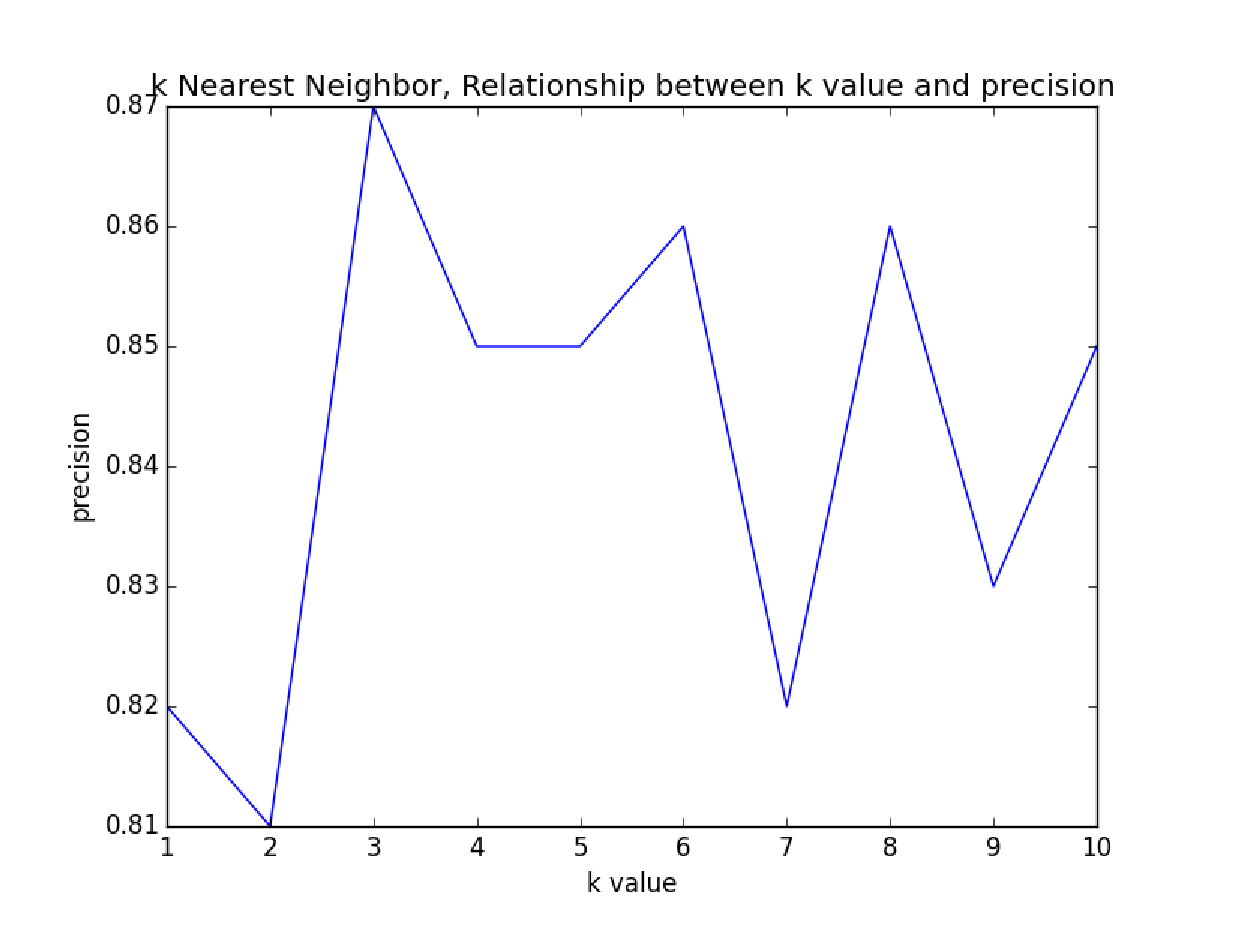
\includegraphics[width=0.8\textwidth]{./assets/kadai3_various_kvalue_20150121_231435.eps}
  \caption{k値とLOO法によるkNNの識別率の関係}
  \label{fig:kadai3}
\end{figure}
図\ref{fig:kadai3}より,kが3の時に最も識別性能が高くなっていることが
わかる.

